
%% bare_conf.tex
%% V1.3
%% 2007/01/11
%% by Michael Shell
%% See:
%% http://www.michaelshell.org/
%% for current contact information.
%%
%% This is a skeleton file demonstrating the use of IEEEtran.cls
%% (requires IEEEtran.cls version 1.7 or later) with an IEEE conference paper.
%%
%% Support sites:
%% http://www.michaelshell.org/tex/ieeetran/
%% http://www.ctan.org/tex-archive/macros/latex/contrib/IEEEtran/
%% and
%% http://www.ieee.org/

%%*************************************************************************
%% Legal Notice:
%% This code is offered as-is without any warranty either expressed or
%% implied; without even the implied warranty of MERCHANTABILITY or
%% FITNESS FOR A PARTICULAR PURPOSE! 
%% User assumes all risk.
%% In no event shall IEEE or any contributor to this code be liable for
%% any damages or losses, including, but not limited to, incidental,
%% consequential, or any other damages, resulting from the use or misuse
%% of any information contained here.
%%
%% All comments are the opinions of their respective authors and are not
%% necessarily endorsed by the IEEE.
%%
%% This work is distributed under the LaTeX Project Public License (LPPL)
%% ( http://www.latex-project.org/ ) version 1.3, and may be freely used,
%% distributed and modified. A copy of the LPPL, version 1.3, is included
%% in the base LaTeX documentation of all distributions of LaTeX released
%% 2003/12/01 or later.
%% Retain all contribution notices and credits.
%% ** Modified files should be clearly indicated as such, including  **
%% ** renaming them and changing author support contact information. **
%%
%% File list of work: IEEEtran.cls, IEEEtran_HOWTO.pdf, bare_adv.tex,
%%                    bare_conf.tex, bare_jrnl.tex, bare_jrnl_compsoc.tex
%%*************************************************************************

% *** Authors should verify (and, if needed, correct) their LaTeX system  ***
% *** with the testflow diagnostic prior to trusting their LaTeX platform ***
% *** with production work. IEEE's font choices can trigger bugs that do  ***
% *** not appear when using other class files.                            ***
% The testflow support page is at:
% http://www.michaelshell.org/tex/testflow/



% Note that the a4paper option is mainly intended so that authors in
% countries using A4 can easily print to A4 and see how their papers will
% look in print - the typesetting of the document will not typically be
% affected with changes in paper size (but the bottom and side margins will).
% Use the testflow package mentioned above to verify correct handling of
% both paper sizes by the user's LaTeX system.
%
% Also note that the "draftcls" or "draftclsnofoot", not "draft", option
% should be used if it is desired that the figures are to be displayed in
% draft mode.
%
\documentclass[conference]{IEEEtran}
% Add the compsoc option for Computer Society conferences.
%
% If IEEEtran.cls has not been installed into the LaTeX system files,
% manually specify the path to it like:
% \documentclass[conference]{../sty/IEEEtran}





% Some very useful LaTeX packages include:
% (uncomment the ones you want to load)


% *** MISC UTILITY PACKAGES ***
%
%\usepackage{ifpdf}
% Heiko Oberdiek's ifpdf.sty is very useful if you need conditional
% compilation based on whether the output is pdf or dvi.
% usage:
% \ifpdf
%   % pdf code
% \else
%   % dvi code
% \fi
% The latest version of ifpdf.sty can be obtained from:
% http://www.ctan.org/tex-archive/macros/latex/contrib/oberdiek/
% Also, note that IEEEtran.cls V1.7 and later provides a builtin
% \ifCLASSINFOpdf conditional that works the same way.
% When switching from latex to pdflatex and vice-versa, the compiler may
% have to be run twice to clear warning/error messages.






% *** CITATION PACKAGES ***
%
%\usepackage{cite}
% cite.sty was written by Donald Arseneau
% V1.6 and later of IEEEtran pre-defines the format of the cite.sty package
% \cite{} output to follow that of IEEE. Loading the cite package will
% result in citation numbers being automatically sorted and properly
% "compressed/ranged". e.g., [1], [9], [2], [7], [5], [6] without using
% cite.sty will become [1], [2], [5]--[7], [9] using cite.sty. cite.sty's
% \cite will automatically add leading space, if needed. Use cite.sty's
% noadjust option (cite.sty V3.8 and later) if you want to turn this off.
% cite.sty is already installed on most LaTeX systems. Be sure and use
% version 4.0 (2003-05-27) and later if using hyperref.sty. cite.sty does
% not currently provide for hyperlinked citations.
% The latest version can be obtained at:
% http://www.ctan.org/tex-archive/macros/latex/contrib/cite/
% The documentation is contained in the cite.sty file itself.






% *** GRAPHICS RELATED PACKAGES ***
%
\ifCLASSINFOpdf
  % \usepackage[pdftex]{graphicx}
  % declare the path(s) where your graphic files are
  % \graphicspath{{../pdf/}{../jpeg/}}
  % and their extensions so you won't have to specify these with
  % every instance of \includegraphics
  % \DeclareGraphicsExtensions{.pdf,.jpeg,.png}
\else
  % or other class option (dvipsone, dvipdf, if not using dvips). graphicx
  % will default to the driver specified in the system graphics.cfg if no
  % driver is specified.
  % \usepackage[dvips]{graphicx}
  % declare the path(s) where your graphic files are
  % \graphicspath{{../eps/}}
  % and their extensions so you won't have to specify these with
  % every instance of \includegraphics
  % \DeclareGraphicsExtensions{.eps}
\fi
% graphicx was written by David Carlisle and Sebastian Rahtz. It is
% required if you want graphics, photos, etc. graphicx.sty is already
% installed on most LaTeX systems. The latest version and documentation can
% be obtained at: 
% http://www.ctan.org/tex-archive/macros/latex/required/graphics/
% Another good source of documentation is "Using Imported Graphics in
% LaTeX2e" by Keith Reckdahl which can be found as epslatex.ps or
% epslatex.pdf at: http://www.ctan.org/tex-archive/info/
%
% latex, and pdflatex in dvi mode, support graphics in encapsulated
% postscript (.eps) format. pdflatex in pdf mode supports graphics
% in .pdf, .jpeg, .png and .mps (metapost) formats. Users should ensure
% that all non-photo figures use a vector format (.eps, .pdf, .mps) and
% not a bitmapped formats (.jpeg, .png). IEEE frowns on bitmapped formats
% which can result in "jaggedy"/blurry rendering of lines and letters as
% well as large increases in file sizes.
%
% You can find documentation about the pdfTeX application at:
% http://www.tug.org/applications/pdftex

\usepackage{graphicx}
\usepackage{tabularx}
\usepackage[strings]{underscore}
\usepackage{fixltx2e}
\usepackage{eurosym}

% *** MATH PACKAGES ***
%
%\usepackage[cmex10]{amsmath}
% A popular package from the American Mathematical Society that provides
% many useful and powerful commands for dealing with mathematics. If using
% it, be sure to load this package with the cmex10 option to ensure that
% only type 1 fonts will utilized at all point sizes. Without this option,
% it is possible that some math symbols, particularly those within
% footnotes, will be rendered in bitmap form which will result in a
% document that can not be IEEE Xplore compliant!
%
% Also, note that the amsmath package sets \interdisplaylinepenalty to 10000
% thus preventing page breaks from occurring within multiline equations. Use:
%\interdisplaylinepenalty=2500
% after loading amsmath to restore such page breaks as IEEEtran.cls normally
% does. amsmath.sty is already installed on most LaTeX systems. The latest
% version and documentation can be obtained at:
% http://www.ctan.org/tex-archive/macros/latex/required/amslatex/math/





% *** SPECIALIZED LIST PACKAGES ***
%
%\usepackage{algorithmic}
% algorithmic.sty was written by Peter Williams and Rogerio Brito.
% This package provides an algorithmic environment fo describing algorithms.
% You can use the algorithmic environment in-text or within a figure
% environment to provide for a floating algorithm. Do NOT use the algorithm
% floating environment provided by algorithm.sty (by the same authors) or
% algorithm2e.sty (by Christophe Fiorio) as IEEE does not use dedicated
% algorithm float types and packages that provide these will not provide
% correct IEEE style captions. The latest version and documentation of
% algorithmic.sty can be obtained at:
% http://www.ctan.org/tex-archive/macros/latex/contrib/algorithms/
% There is also a support site at:
% http://algorithms.berlios.de/index.html
% Also of interest may be the (relatively newer and more customizable)
% algorithmicx.sty package by Szasz Janos:
% http://www.ctan.org/tex-archive/macros/latex/contrib/algorithmicx/




% *** ALIGNMENT PACKAGES ***
%
%\usepackage{array}
% Frank Mittelbach's and David Carlisle's array.sty patches and improves
% the standard LaTeX2e array and tabular environments to provide better
% appearance and additional user controls. As the default LaTeX2e table
% generation code is lacking to the point of almost being broken with
% respect to the quality of the end results, all users are strongly
% advised to use an enhanced (at the very least that provided by array.sty)
% set of table tools. array.sty is already installed on most systems. The
% latest version and documentation can be obtained at:
% http://www.ctan.org/tex-archive/macros/latex/required/tools/


%\usepackage{mdwmath}
%\usepackage{mdwtab}
% Also highly recommended is Mark Wooding's extremely powerful MDW tools,
% especially mdwmath.sty and mdwtab.sty which are used to format equations
% and tables, respectively. The MDWtools set is already installed on most
% LaTeX systems. The lastest version and documentation is available at:
% http://www.ctan.org/tex-archive/macros/latex/contrib/mdwtools/


% IEEEtran contains the IEEEeqnarray family of commands that can be used to
% generate multiline equations as well as matrices, tables, etc., of high
% quality.


%\usepackage{eqparbox}
% Also of notable interest is Scott Pakin's eqparbox package for creating
% (automatically sized) equal width boxes - aka "natural width parboxes".
% Available at:
% http://www.ctan.org/tex-archive/macros/latex/contrib/eqparbox/





% *** SUBFIGURE PACKAGES ***
%\usepackage[tight,footnotesize]{subfigure}
% subfigure.sty was written by Steven Douglas Cochran. This package makes it
% easy to put subfigures in your figures. e.g., "Figure 1a and 1b". For IEEE
% work, it is a good idea to load it with the tight package option to reduce
% the amount of white space around the subfigures. subfigure.sty is already
% installed on most LaTeX systems. The latest version and documentation can
% be obtained at:
% http://www.ctan.org/tex-archive/obsolete/macros/latex/contrib/subfigure/
% subfigure.sty has been superceeded by subfig.sty.



%\usepackage[caption=false]{caption}
%\usepackage[font=footnotesize]{subfig}
% subfig.sty, also written by Steven Douglas Cochran, is the modern
% replacement for subfigure.sty. However, subfig.sty requires and
% automatically loads Axel Sommerfeldt's caption.sty which will override
% IEEEtran.cls handling of captions and this will result in nonIEEE style
% figure/table captions. To prevent this problem, be sure and preload
% caption.sty with its "caption=false" package option. This is will preserve
% IEEEtran.cls handing of captions. Version 1.3 (2005/06/28) and later 
% (recommended due to many improvements over 1.2) of subfig.sty supports
% the caption=false option directly:
%\usepackage[caption=false,font=footnotesize]{subfig}
%
% The latest version and documentation can be obtained at:
% http://www.ctan.org/tex-archive/macros/latex/contrib/subfig/
% The latest version and documentation of caption.sty can be obtained at:
% http://www.ctan.org/tex-archive/macros/latex/contrib/caption/




% *** FLOAT PACKAGES ***
%
%\usepackage{fixltx2e}
% fixltx2e, the successor to the earlier fix2col.sty, was written by
% Frank Mittelbach and David Carlisle. This package corrects a few problems
% in the LaTeX2e kernel, the most notable of which is that in current
% LaTeX2e releases, the ordering of single and double column floats is not
% guaranteed to be preserved. Thus, an unpatched LaTeX2e can allow a
% single column figure to be placed prior to an earlier double column
% figure. The latest version and documentation can be found at:
% http://www.ctan.org/tex-archive/macros/latex/base/



%\usepackage{stfloats}
% stfloats.sty was written by Sigitas Tolusis. This package gives LaTeX2e
% the ability to do double column floats at the bottom of the page as well
% as the top. (e.g., "\begin{figure*}[!b]" is not normally possible in
% LaTeX2e). It also provides a command:
%\fnbelowfloat
% to enable the placement of footnotes below bottom floats (the standard
% LaTeX2e kernel puts them above bottom floats). This is an invasive package
% which rewrites many portions of the LaTeX2e float routines. It may not work
% with other packages that modify the LaTeX2e float routines. The latest
% version and documentation can be obtained at:
% http://www.ctan.org/tex-archive/macros/latex/contrib/sttools/
% Documentation is contained in the stfloats.sty comments as well as in the
% presfull.pdf file. Do not use the stfloats baselinefloat ability as IEEE
% does not allow \baselineskip to stretch. Authors submitting work to the
% IEEE should note that IEEE rarely uses double column equations and
% that authors should try to avoid such use. Do not be tempted to use the
% cuted.sty or midfloat.sty packages (also by Sigitas Tolusis) as IEEE does
% not format its papers in such ways.





% *** PDF, URL AND HYPERLINK PACKAGES ***
%
%\usepackage{url}
% url.sty was written by Donald Arseneau. It provides better support for
% handling and breaking URLs. url.sty is already installed on most LaTeX
% systems. The latest version can be obtained at:
% http://www.ctan.org/tex-archive/macros/latex/contrib/misc/
% Read the url.sty source comments for usage information. Basically,
% \url{my_url_here}.





% *** Do not adjust lengths that control margins, column widths, etc. ***
% *** Do not use packages that alter fonts (such as pslatex).         ***
% There should be no need to do such things with IEEEtran.cls V1.6 and later.
% (Unless specifically asked to do so by the journal or conference you plan
% to submit to, of course. )


% correct bad hyphenation here
\hyphenation{op-tical net-works semi-conduc-tor}


\begin{document}
%
% paper title
% can use linebreaks \\ within to get better formatting as desired
\title{Towards a smart city: An air quality monitoring system in Perheim}


% author names and affiliations
% use a multiple column layout for up to three different
% affiliations
\author{\IEEEauthorblockN{Henrik Lechte, Florian Finkel, Julia Grabinski, Cara Damm}
\IEEEauthorblockA{University of Mannheim\\
Pervasive Computing: Smart City Air Quality Sensors - FSS 2019\\
Master of Business Informatics\\ 
Email: \{first name\}.\{last name\}@mail.uni-mannheim.de}
}

% conference papers do not typically use \thanks and this command
% is locked out in conference mode. If really needed, such as for
% the acknowledgment of grants, issue a \IEEEoverridecommandlockouts
% after \documentclass

% for over three affiliations, or if they all won't fit within the width
% of the page, use this alternative format:
% 
%\author{\IEEEauthorblockN{Michael Shell\IEEEauthorrefmark{1},
%Homer Simpson\IEEEauthorrefmark{2},
%James Kirk\IEEEauthorrefmark{3}, 
%Montgomery Scott\IEEEauthorrefmark{3} and
%Eldon Tyrell\IEEEauthorrefmark{4}}
%\IEEEauthorblockA{\IEEEauthorrefmark{1}School of Electrical and Computer Engineering\\
%Georgia Institute of Technology,
%Atlanta, Georgia 30332--0250\\ Email: see http://www.michaelshell.org/contact.html}
%\IEEEauthorblockA{\IEEEauthorrefmark{2}Twentieth Century Fox, Springfield, USA\\
%Email: homer@thesimpsons.com}
%\IEEEauthorblockA{\IEEEauthorrefmark{3}Starfleet Academy, San Francisco, California 96678-2391\\
%Telephone: (800) 555--1212, Fax: (888) 555--1212}
%\IEEEauthorblockA{\IEEEauthorrefmark{4}Tyrell Inc., 123 Replicant Street, Los Angeles, California 90210--4321}}




% use for special paper notices
%\IEEEspecialpapernotice{(Invited Paper)}




% make the title area
\maketitle
\thispagestyle{plain}
\pagestyle{plain}


\begin{abstract}
%\boldmath
\end{abstract}
% IEEEtran.cls defaults to using nonbold math in the Abstract.
% This preserves the distinction between vectors and scalars. However,
% if the conference you are submitting to favors bold math in the abstract,
% then you can use LaTeX's standard command \boldmath at the very start
% of the abstract to achieve this. Many IEEE journals/conferences frown on
% math in the abstract anyway.

% no keywords




% For peer review papers, you can put extra information on the cover
% page as needed:
% \ifCLASSOPTIONpeerreview
% \begin{center} \bfseries EDICS Category: 3-BBND \end{center}
% \fi
%
% For peerreview papers, this IEEEtran command inserts a page break and
% creates the second title. It will be ignored for other modes.
\IEEEpeerreviewmaketitle

\section{Introduction}

Air quality is a topic which is facing much publicity due to its prevalence in law and media, especially regarding pollution laws leading to driving bans. Poor air quality caused by industry and daily life leads to health risks and adversely impacts the environment. Inhabitants of big cities are particularly affected by air pollutants, which might manifest themselves in smog or an industrial smell.
Meanwhile, the concept of internet of things devices is on the rise, enabled by increased computation power, cost and energy efficient sensors and the availability of a fast cellular network.
\newline
Due to this, the city of Perheim may want to consider to implement an air quality control system based on a multitude of sensors in a connected network. Thereby, aggregated and location-based information about the current air quality can be provided.

\section{Existing approaches}
It should be noted that measuring air quality as part of a smart city is no new approach, but has already been discussed in research \cite{Nagaraj} and has also been implemented in real-world projects. This shows that an air quality information system is a relevant topic. However, the concept for the city of Perheim is not directly based on one of these approaches. Existing research ranges for example from the application of low-cost crowd sensing sensors \cite{Dutta} to the combination of sensors with video monitoring of traffic \cite{Mehta} as well as using neural nets to predict future air pollution values \cite{Kok}. Real-world projects include the London air quality network (LAQN) launched in 1993 \cite{Mittal.2018} and the so-called Array of Things in Chicago consisting of lamppost-mounted sensors \cite{Adler.2015}.

There is also already a basic air monitoring system in place in the Rhein-Neckar area \cite{LandesanstaltfurUmweltBadenWurttemberg}.
However, the new smart city air quality concept for Perheim differs in several aspects from the already existing system of the Rhein-Neckar area:
\begin{itemize} 
\item The existing air monitoring consists of very few sensors per area. However, the approach propsed in this paper makes use of a higher number of small sensors to enable fine-granular monitoring.
\item A new interconnected approach also allows for futher integrating more sophisticated smart city concepts regarding automatic traffic diversion and health care in the future.
\item Currently, the measurements are not easy to consume. With live monitoring and an intuitive user interface, the visibility of the current status of the air quality will be greatly improved for citizens.
\end{itemize} 

\section{Use cases}
Monitoring the air quality and providing information directly might prove useful in differerent use cases. It is also important to note that air quality is a very relevant topic for the city of Perheim. Perheim's downtown area is heavily frequented by cars. Furthermore, one of the world's biggest chemical companies, whose emissions and increased risk of toxic accidents and fires might also adversely impact the air quality, is headquartered in the neighboring city.
\newline \newline
Each of the following use cases can be enabled by an air quality information system. The required technology and sensors will be covered in section \ref{sec:TechnicalImplementation}.

\subsection{Managing health risks}
With an air quality information system, citizens can base their decision of when to leave the house or where to go for daily-life activities on the air quality. This might prove to be especially helpful for people with severe allergies or other adverse reactions to air pollutants. Also, health institutions can use the data and the home address of a patient to possibly correlate health issues with air pollution and thus providing more precise diagnosis. The air quality information system can also be used to give direct feedback in case of an acute risk by wildfires or leaks at chemical plants. In both cases it is usually recommended to stay inside. Negative health risks resulting from a high concentration of some air pollutants are summarized in a report carried out by the World Health Organization and are as follows \cite{WorldHealthOrganization.2013}:

\begin{description} 
\item[O\textsubscript{3}] Long- and short-term excessive ozone exposure can lead to respiratory diseases and restrictions in activity.
\item[NO\textsubscript{2}] Nitrogen dioxide exposure can lead to bronchitic symptoms in asthmatic children as well as an increase in all-cause mortality.
\item[PM\textsubscript{2.5}] Long-term effects of excessive exposure to particulate matter of 2.5 micrometers or less can be cardiovascular diseases, lung cancer and an increased all-cause mortality.
\item[PM\textsubscript{10}] Inhaling particulate matter of 10 micrometers or less may result in asthma symptoms in asthmatic children and chronic bronchitis.
\end{description} 

Apart from these major air pollutants, there is a wide variety of other air toxics which may cause cancer, respiratory reactions or other diseases \cite{UnitedStatesEnvironmentalProtectionAgency}.

It is also possible to  build on the air quality information system by integrating the generated data into other technical devices. For example, windows could be automatically closed, air filters regulated and car navigation system could propose routes based on the air quality. However, this is out-of-scope for a first technical implementation in Perheim.

\subsection{Environmental damage}
Poor air quality not only impacts human health, but also the well-being of animals and plants. While the population of economically valuable insects can decline due to poor air quality, it could be observed that certain types of unwanted insects benefit from air pollutants \cite{Dohmen.1984}\cite{Alstad.1982}. The presence of air pollutants also reduces plant growth \cite{CRITTENDEN.1978}. One of the major factors for this dynamic was sulfor dioxide causing acid rain. However, the sulfor dioxide emissions declined by 90\%in Germany since 1990 making this not as much of a problem as three decades ago \cite{Umweltbundesamt.01.05.2019}.

However, there is still a multitude of other pollutants affecting the environment \cite{Umweltbundesamt.2018}\cite{UnitedStatesEnvironmentalProtectionAgency.01.05.2019}.

In this context, the air quality information system can be used to investigate changes in the eco-system, to monitor the impact of the location of plants and roads and to find suitable locations to grow organic food.

\subsection{Enabling law execution}
The impact of poor air quality on health and the environment has also been recognized by law makers. There are several laws governing the air pollution for industry and car traffic. The most important EU directive is 2008/50/EC \cite{EurpoeanUnion.2008}. This directive provides legal limit values for certain pollutants such as particulate matter, nitrogen dioxide and carbon monoxide. An air quality control system can help to monitor these limits, take action when needed and control their execution. Unusual or extreme measurements also hint on law breaches for example in form of illegaly operarted facilities that are subject to approval. In this case, the local municipality is allowed to take action in compliance with \S20 and \S62 of the Bundes-Immissionsschutzgesetz (BImSchG) \cite{BundesrepublikDeutschland.1974}. In a more advanced smart city approach, the fine-granular air quality information will be integrated automatic traffic control. Thereby, automatic speed limits and the diversion of cars from heavily to less frequented areas and streets help to satisfy required pollution limits.

\subsection{Psychological effect}
Having a direct and real-time exposure to air quality data might result in an increased ecological awareness of citizens. Thereby, a voluntary switch from e.g. coal energy to a renewable energy provider or from environmental-unfriendly cars to electric vehicles might be initiated. In the same context, Perheim receives an image boost, showing the city as being environmental friendly and digitally advanced.

\section{Economic feasability}
While the initial cost of sensors is not expected to be exceptionally high, maintenance and installation must also be accounted for. Several different models to covering the costs are possible.

\subsection{Tax-payer funded service}
In the most straight-forward approach, the local municipality and thus indirectly the tax payer is responsible for buying and installing the sensors. The service is then provided to all citizens of Perheim free of charge. This is a sensible idea because not only do the citizens benefit from the air quality information system, but also the municipality itself.

\subsection{Subscription-based service}
Like other cloud and internet of things services, the air quality information could be provided as a subscription for a small fee of a few euros per month. However, this bears the disadvantage that most people might not be interested in the service or do not consider the price-value ratio as attractive. It could also be possible to keep some measured values free and enabling additional information based on more specific sensors for a small fee.
As discussed before, an air quality information system could be used as a foundation for other products such as smart home devices and health care software. Therefore, a seperate subscription for commercial use might be reasonable.

\subsection{Voluntary contributions}
The sensors could also be sold to the citizens at a discount. Thereby, Perheim's inhabitants can contribute voluntarily by buying the sensors and installing them outside their home. Through this model, a fine granular network can be achieved and the city only needs to cover the costs for the discount and servers. However, this approach entirely relies on a wide participation rate in the population.

\subsection{Data as a product}
Historical and live data might be interesting for companies and researches. Selling complete data sets might complement one of the other models. 


\section{Technical implementation} \label{sec:TechnicalImplementation}
In terms of technical implementation of the first generation of an air quality information system, the goal is to reduce costs and keep the technical aspects simple. Therefore, the air quality sensor will be built using an Arduino and multiple other sensors. Afterwards, numerous of these air quality sensors will be installed in Perheim. Following the installation, the measured data is loaded into a central database and displayed in an easy to use and visually appealing application. The following chapters will cover a possible implementation of each of these steps in detail.

\subsection{Building the air quality sensor}
First of all, it has to be determined what the final air quality sensor should measure. The European Union defined the European Air Quality Index (EAQI) in 2017 and it is similar to most of the Air Quality Index from other governments around the world, like the U.S. Environmental Protection Agency (EPA). It provides a set of air quality index levels: good, fair, moderate, poor and very poor. Furthermore, it defines multiple components, such as ozone, particulate matter, sulfur dioxide, carbon monoxide and nitrous oxide, that are getting measured and it provides a table to calculate the EAQI with the measured data of these components. Since the EAQI covers most of the important pollutants and is used throughout Europe, it will serve as the basis for the air quality sensors in Perheim (Germany). As the goal is to distribute a multitude of air quality sensors in Perheim, the first generation of air quality sensors will be built with inexpensive sensors to make them more affordable. In a later stage, when the developed system proves to be useful, sensors can be more expensive and of higher quality. With the focus on reducing the costs, the following sensors will be used for the first-generation air quality sensors:

\begin{itemize}
\item Ozone: \textit{SainSmart MQ131}
\item Particulate matter: \textit{Grove Dust Sensor}
\item Sulfur dioxide: \textit{Mq2 Gas Sensor}
\item Carbon monoxide: \textit{Mq9 Gas Sensor}
\item Nitrous oxide: \textit{MICS-2714}
\end{itemize}

With these sensors all the components of the EAQI can be measured. Other important factors that play an essential role to the severeness of the EAQI are the current temperature and humidity. This is why a temperature and humidity sensor will also be integrated into the air quality sensor to improve the calculations. In the first iteration the \textit{SODIAL - Temperature and Relative Humidity Sensor} will be used. Another important feature is, that the final application has to use the location of each sensor to display the measured data at the corresponding site. Therefore, each air quality sensor will be equipped with a \textit{NEO-6M GPS} sensor to send the Global Positioning System (GPS) coordinates of its location with each measured data set. At last, the internet module \textit{FONA Mini Cell GSM Breakout SMA} will be utilized to connect the Arduino to the internet and send the measured sensor data to a central system for further processing. All these hardware components will be soldered to a soldering board and thereby connected to the Arduino. The final construct will be placed in a weatherproof box that has three cutouts. A 5-Volt fan will be placed in the first cutout to blow the air through the box, along all the sensors and finally out of the second cutout. The third cutout is for a power supply for the Arduino. All initial air quality sensors will be manufactured using the procedure. The estimated cost of one sensor without the box is approximately 150 \euro. The required Arduino coding to read all the measurements is not part of this document.

\subsection{Creating a backend to process incoming data and managing already placed air quality sensors}
The backend system that provides an application programming interface (API) for each interaction type with both air quality sensors and the frontend application will be covered in this section. These APIs can be implemented in many ways, e.g. as a Representational State Transfer (REST) APIs or as a create, read, update, and delete (CRUD) APIs, but the detailed implementation of these APIe won’t be discussed in this document. The first API will receive the sent measurements of the air quality sensors and will provide the following functionalities:
\begin{itemize}
\item Receive a set of data containing the measurements, a timestamp and location from a sensor in JavaScript Object Notation (JSON) format
\item Save received data into a persistence as one tuple of the corresponding database table
\item Error handling in the event of wrong message formats
\item Propagate crucial information if sensor measurements could be hazardous to health
\item Authorization and authentication checks for each request
\end{itemize}
Moreover, the backend will also provide another API that sensors can poll from to retrieve the current interval time for sensor measurements. In case of numerous distributed sensors this API will make it easy to adjust said interval and avoid unnecessary manual labour. It will provide these features:
\begin{itemize}
\item Accept GET requests and return the currently set measurement interval
\item Accept PUT and POST request to set a new measurement interval
\item Error handling in case of a wrong request format
\item Authorization and authentication checks for each request
\end{itemize}
With the two APIs defined before all the required interactions between each air quality sensor and the backend can be achieved.

Since these two backend endpoints should provide authorization and authentication checks, a corresponding security system has to be implemented. For the first generation sensors the widely established open standard OAuth 2.0 will be utilized. Therefore, the backend system will provide an authorization server that returns access tokens for the sensors. When a sensor is build the OAuth client credentials flow has to be performed manually to retrieve an access token for the new sensor. After receiving the token it will be hardcoded into the sensor which will in return send this token in each of its measurement requests as authorization header. Figure \ref{fig:credentialsFlow} illustrates this concept in a simplified representation.

\begin{figure}[htbp]
	\centering
	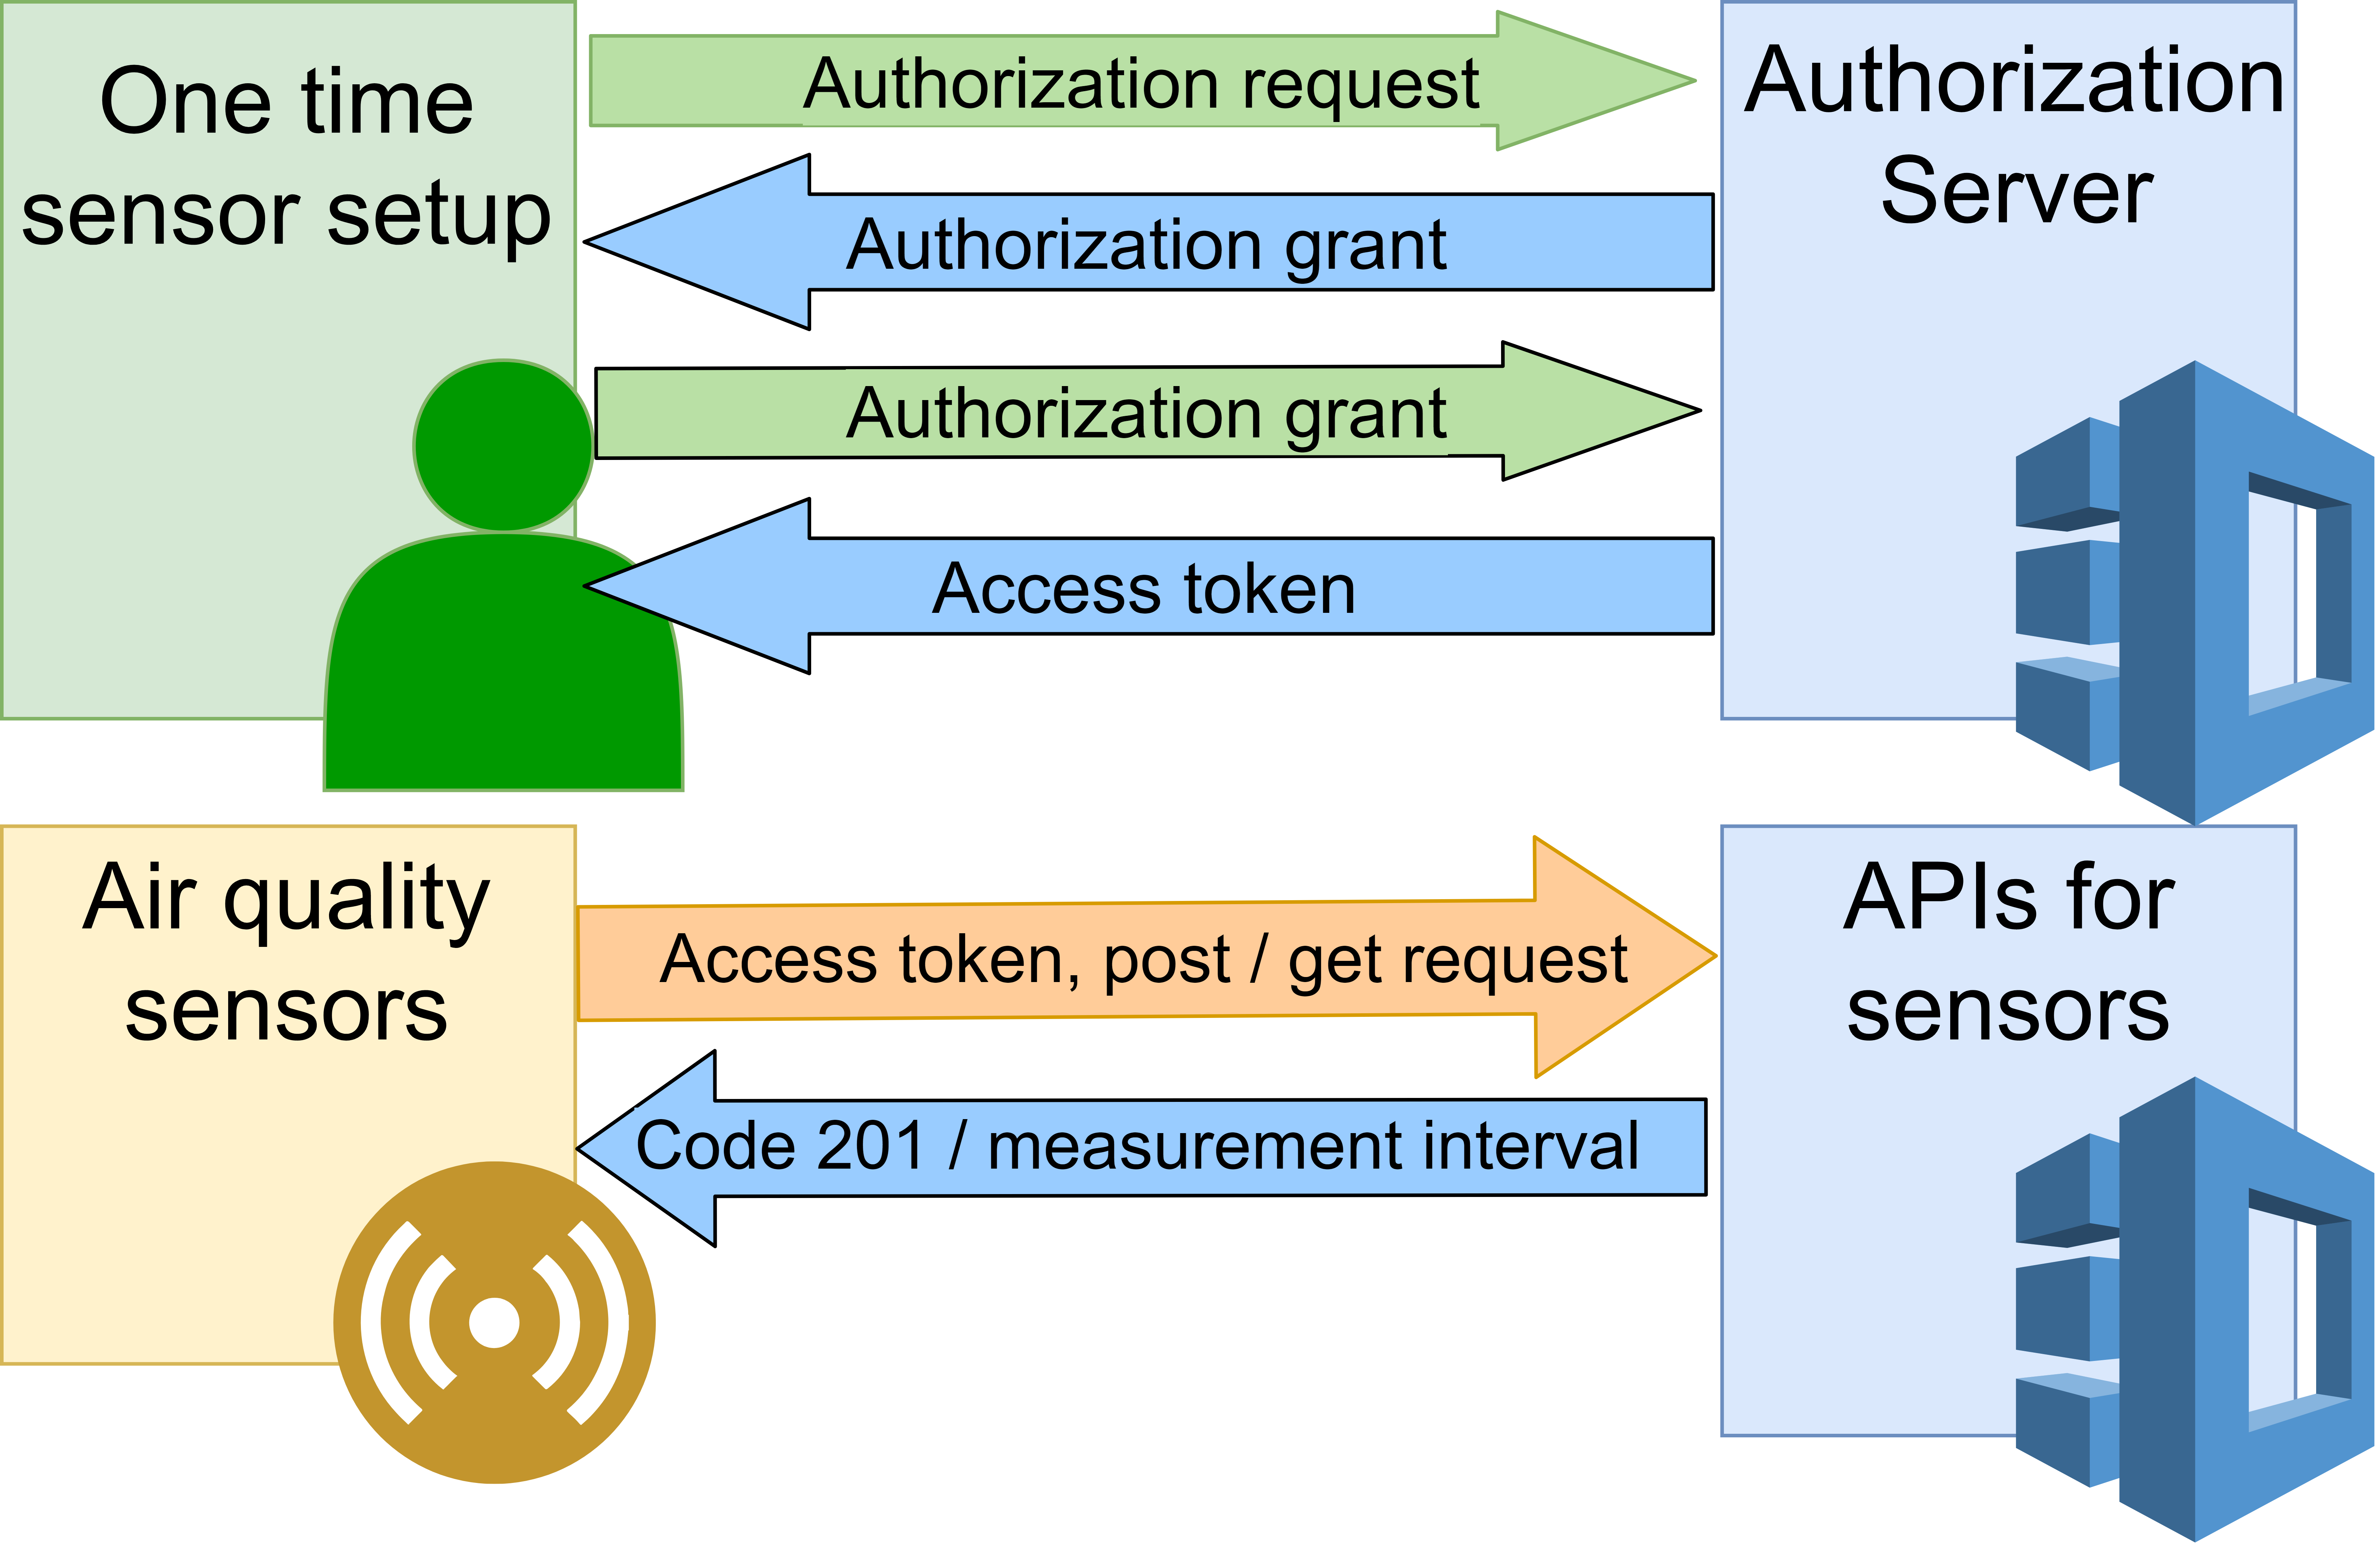
\includegraphics[width=0.48\textwidth]{AirQualityOAuthCredentialsFlow.png}
	\caption{Air quality sensor OAuth credentials flow}
	\label{fig:credentialsFlow}
\end{figure}

Usually OAuth access tokens have an expiration date but for the first generation sensors each token can be used for an unlimited time period. In a later implementation phase the security concept should be reworked since the manual set up is tedious and using an access token for a prolonged time may result in security vulnerabilities. Such a security rework could include an oauth credentials flow automation where each sensor retrieves itself new access tokens in a set time intervalA without manual working steps.

Lastly an API for the frontend will be created. Here the following features are required:
\begin{itemize}
\item Retrieve measured air quality level and location of each sensor
\item Error handling in case of wrong request format
\item Authorization and authentication checks for each request 
\end{itemize}
With the previously explained APIs the backend system includes the necessary functionalities for all interactions for both the air quality sensors and the frontend.


\subsection{Creating the frontend application}
A map overview of Perheim will be provided:
\begin{figure}[htbp]
	\centering
	\includegraphics[width=0.48\textwidth]{perheimMapMockup.png}
	\caption{perheimMapMockup}
	\label{fig:credentialsFlow}
\end{figure}

Detailed measurements of each sensor will be provided:
\begin{figure}[htbp]
	\centering
	\includegraphics[width=0.48\textwidth]{DetailedSensorMeasurementsMockup.png}
	\caption{DetailedSensorMeasurementsMockup}
	\label{fig:credentialsFlow}
\end{figure}

Notifications will be provided but no MockUp :>

\section{Conclusion}
The implementation of an air quality information system in Perheim appears to be a reasonable concept. Through constant monitoring of various air pollutants, health risks can be reduced, environmental effects observed and laws enforced. By using inexpensive components and a simple archtitecture, costs are reduced and a first pilot implementation can be performed with comparitvely low effort. The first implementation serves as a foundation for a later extension with more sophisticated technology as well as integration to other smart home and city concepts. 




% conference papers do not normally have an appendix


% use section* for acknowledgement


% trigger a \newpage just before the given reference
% number - used to balance the columns on the last page
% adjust value as needed - may need to be readjusted if
% the document is modified later
%\IEEEtriggeratref{8}
% The "triggered" command can be changed if desired:
%\IEEEtriggercmd{\enlargethispage{-5in}}

% references section

% can use a bibliography generated by BibTeX as a .bbl file
% BibTeX documentation can be easily obtained at:
% http://www.ctan.org/tex-archive/biblio/bibtex/contrib/doc/
% The IEEEtran BibTeX style support page is at:
% http://www.michaelshell.org/tex/ieeetran/bibtex/
%\bibliographystyle{IEEEtran}
% argument is your BibTeX string definitions and bibliography database(s)
%\bibliography{IEEEabrv,../bib/paper}
%
% <OR> manually copy in the resultant .bbl file
% set second argument of \begin to the number of references
% (used to reserve space for the reference number labels box)
%\begin{thebibliography}{1}

%\bibitem{IEEEhowto:kopka}
%H.~Kopka and P.~W. Daly, \emph{A Guide to \LaTeX}, 3rd~ed.\hskip 1em plus
% 0.5em minus 0.4em\relax Harlow, England: Addison-Wesley, 1999.


%\end{thebibliography}

\bibliographystyle{IEEEtran}
\bibliography{literature}



% that's all folks
\end{document}


